\section{Recolección y Ordenamiento de la Información}

\subsection{Fuentes de información}

La recolección combinó cuatro fuentes. La primera fue la API de GitHub, utilizada para identificar candidatos, recuperar metadatos de popularidad y actividad, verificar manifiestos y confirmar la existencia de commits recientes. La segunda fue el código fuente de los repositorios clonados, fijado a un commit específico, que constituye la evidencia primaria para la detección de antipatrones y el cálculo de métricas. La tercera fueron los documentos del proyecto: la taxonomía operacional, las decisiones metodológicas D1--D10, los protocolos de validación y los informes de ejecución. La cuarta fue la literatura científica y técnica sobre antipatrones arquitectónicos, deuda técnica en sistemas de aprendizaje automático, detección estática y arquitecturas RAG.

El período de observación se delimitó con una fecha de corte de un año antes de la extracción. Las consultas exigieron actividad posterior al 23 de noviembre de 2025, de modo que la muestra priorizara proyectos activos y no repositorios abandonados. La extracción de metadatos se realizó el 23 de noviembre de 2026. Esta ventana de doce meses es una decisión de diseño y no una propiedad de los datos: un repositorio activo en ese período pudo haber cambiado después, pero el análisis se realizó sobre la versión fijada por SHA.

\subsection{Universo y cribado}

El universo inicial se construyó con consultas por tópicos asociados a RAG, agentes, LLM y marcos de recuperación, restringidas a Python, sin forks ni repositorios archivados y con al menos once estrellas. Las consultas se distribuyeron en tres bandas de popularidad para evitar que la muestra quedara dominada por proyectos muy grandes. Tras la deduplicación por nombre completo, el universo histórico quedó en 915 candidatos. Los intentos de ampliación mediante consultas agrupadas por tecnologías no devolvieron resultados utilizables antes del límite de búsqueda de la API, por lo que se conservó ese universo y se decidió ampliar el cribado en lugar de ampliar la recolección.

La preselección tomó 120 filas, cuarenta por banda, ordenadas de forma determinista por estrellas y filtradas con palabras clave que excluyen tutoriales, cursos, talleres, listas de recursos, ejemplos, demostraciones, libros de recetas, cuadernos y plantillas. Esta etapa no pretendía decidir la elegibilidad, sino reducir el costo de la verificación. La verificación posterior se aplicó a las 120 filas y comprobó tres condiciones: manifiesto raíz, tecnología asociada a RAG en los manifiestos y al menos veinte commits en el período. El resultado fue de 24 repositorios elegibles y 96 excluidos. Las causas de exclusión se conservaron en un archivo específico y se agrupan en tres familias: ausencia de tecnología RAG en los manifiestos, ausencia de manifiesto raíz y actividad insuficiente en el período.

Los 24 elegibles se clonaron y se sometieron a una verificación local de relevancia. Esta verificación leyó el README y el código en busca de evidencia conjunta de integración de un LLM y de un mecanismo de recuperación, y comparó el SHA clonado con el SHA verificado. Veintitrés repositorios cumplieron; \texttt{Tejas-TA/predikit} fue excluido porque su evidencia no mostraba conjuntamente integración de LLM y recuperación. La muestra final quedó en 23 repositorios. El embudo completo se ilustra en la Figura~\ref{fig:composicion}: 915 candidatos, 120 preseleccionados, 24 elegibles y 23 analizados.

\begin{figure*}[t]
\centering
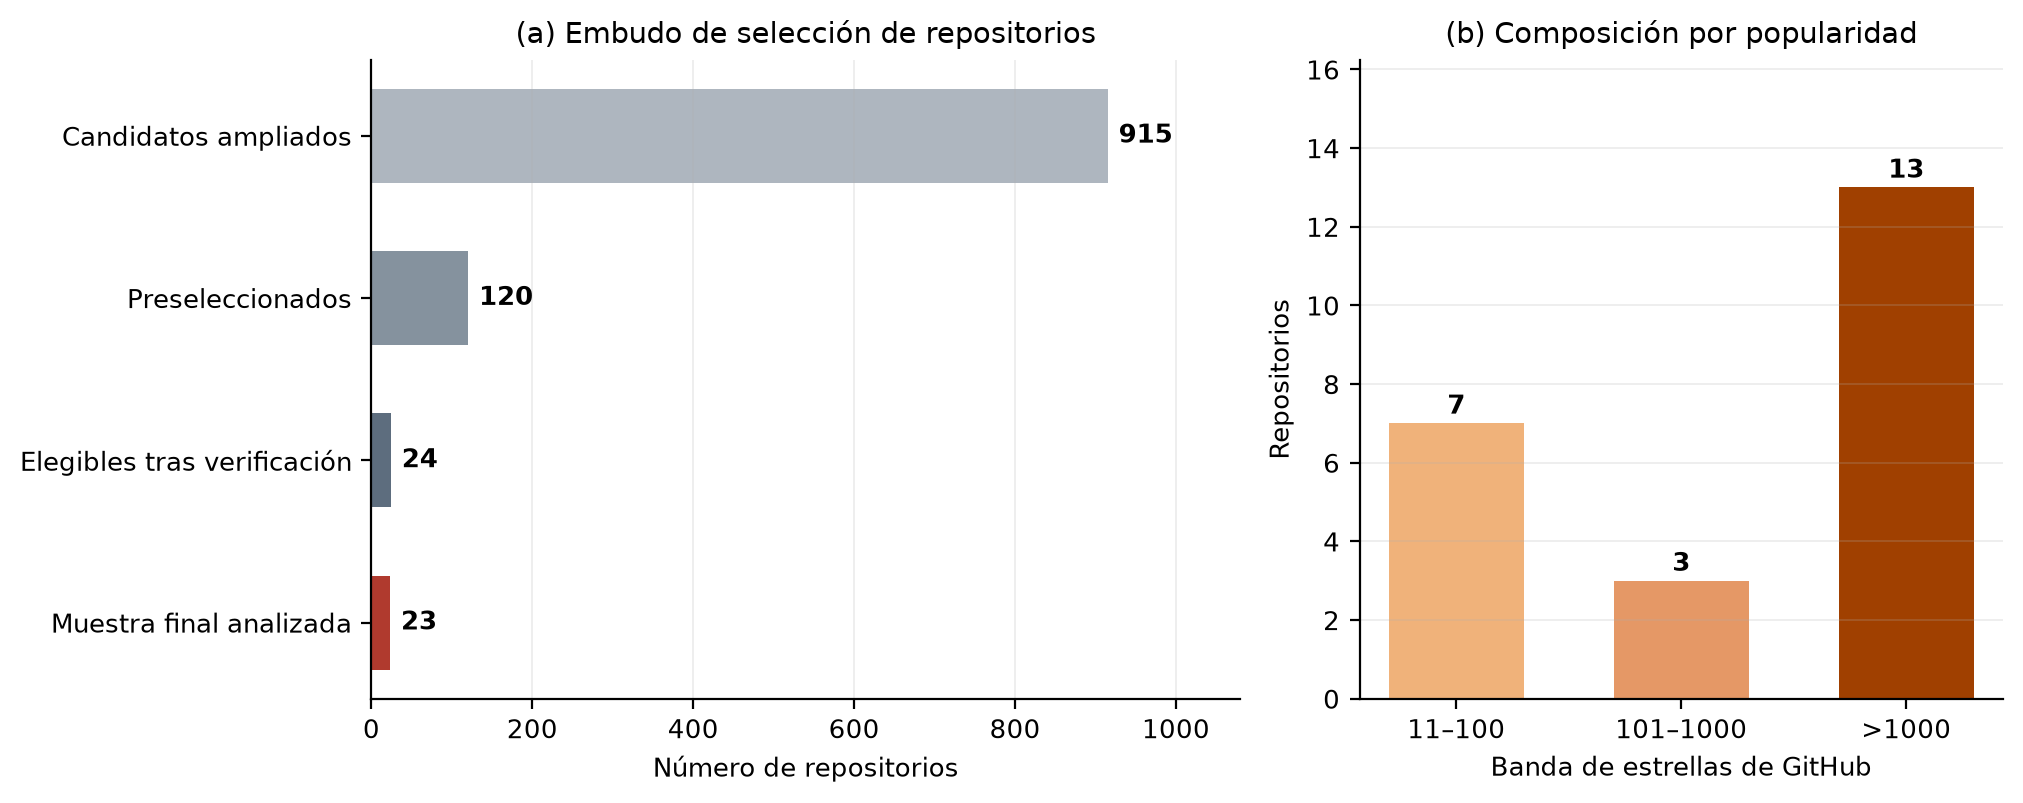
\includegraphics[width=0.92\textwidth]{figuras/fig02_composicion_muestra.png}
\caption{Composición de la muestra. (a) Embudo de selección desde los candidatos ampliados hasta la muestra final. (b) Distribución de los 23 repositorios por banda de estrellas.}
\label{fig:composicion}
\end{figure*}

\subsection{Composición de la muestra}

La Tabla~\ref{tab:muestra} presenta los 23 repositorios con su banda de popularidad, número de módulos elegibles, número de módulos con al menos un hallazgo, porcentaje de módulos afectados y número total de hallazgos. La muestra está desbalanceada por diseño: 13 repositorios pertenecen a la banda de más de 1000 estrellas, 3 a la banda 101--1000 y 7 a la banda 11--100. Este desbalance refleja tanto la disponibilidad de proyectos grandes y activos como el hecho de que la banda superior concentra más candidatos verificables. No se aplicó ponderación para corregirlo, de modo que los resultados describen la muestra tal como quedó constituida y no una población estratificada.

\begin{table*}[t]
\centering
\scriptsize
\setlength{\tabcolsep}{4pt}
\caption{Composición de la muestra: módulos y hallazgos por repositorio}
\label{tab:muestra}
\begin{tabularx}{\textwidth}{@{}X c r r r r@{}}
\toprule
\textbf{Repositorio} & \textbf{Banda} & \textbf{Módulos} & \textbf{Mód.\ con AP} & \textbf{\% con AP} & \textbf{Hallazgos} \\
\midrule
\texttt{multimindlab/multimind-sdk} & 11--100 & 392 & 42 & 10,71 & 194 \\
\texttt{bojieli/ai-agent-book} & >1000 & 1\,037 & 49 & 4,73 & 86 \\
\texttt{ai-bot-pro/achatbot} & 11--100 & 942 & 23 & 2,44 & 27 \\
\texttt{run-llama/llama\_index} & >1000 & 2\,114 & 13 & 0,61 & 21 \\
\texttt{headroomlabs-ai/headroom} & >1000 & 645 & 14 & 2,17 & 21 \\
\texttt{hoangsonww/Agentic-AI-Pipeline} & 11--100 & 73 & 2 & 2,74 & 15 \\
\texttt{onyx-dot-app/onyx} & >1000 & 2\,440 & 9 & 0,37 & 10 \\
\texttt{NJUxlj/Chinese-MedQA-Qwen2} & 11--100 & 137 & 6 & 4,38 & 10 \\
\texttt{arthurpanhku/DocSentinel} & 11--100 & 116 & 2 & 1,72 & 9 \\
\texttt{verygoodplugins/automem} & 101--1000 & 73 & 6 & 8,22 & 7 \\
\texttt{khoj-ai/khoj} & >1000 & 110 & 2 & 1,82 & 7 \\
\texttt{BerriAI/litellm} & >1000 & 3\,601 & 5 & 0,14 & 6 \\
\texttt{mlflow/mlflow} & >1000 & 1\,400 & 4 & 0,29 & 6 \\
\texttt{agentscope-ai/agentscope} & >1000 & 532 & 4 & 0,75 & 5 \\
\texttt{Mattral/filing-qa} & 11--100 & 70 & 5 & 7,14 & 5 \\
\texttt{1Panel-dev/MaxKB} & >1000 & 1\,010 & 5 & 0,50 & 5 \\
\texttt{HKUDS/LightRAG} & >1000 & 204 & 3 & 1,47 & 4 \\
\texttt{Cygnux-Labs/Tracekit} & 101--1000 & 235 & 3 & 1,28 & 3 \\
\texttt{ScrapeGraphAI/Scrapegraph-ai} & >1000 & 140 & 2 & 1,43 & 2 \\
\texttt{mem0ai/mem0} & >1000 & 257 & 1 & 0,39 & 1 \\
\texttt{getzep/graphiti} & >1000 & 210 & 1 & 0,48 & 1 \\
\texttt{ZhishaBai-web/help-you-find-job} & 11--100 & 8 & 0 & 0,00 & 0 \\
\texttt{LibreChat-AI/rag-api} & 101--1000 & 22 & 0 & 0,00 & 0 \\
\midrule
\textbf{Total} & --- & 15\,768 & 201 & 1,27 & 445 \\
\bottomrule
\end{tabularx}
\end{table*}

El tamaño de los repositorios es muy heterogéneo. \texttt{BerriAI/litellm} aporta 3601 módulos, \texttt{onyx-dot-app/onyx} 2440 y \texttt{run-llama/llama\_index} 2114, mientras que \texttt{ZhishaBai-web/help-you-find-job} aporta 8 y \texttt{LibreChat-AI/rag-api} 22. Esta heterogeneidad implica que las comparaciones a nivel de módulo están dominadas por unos pocos repositorios grandes y que los repositorios pequeños tienen poca influencia en los contrastes globales. La concentración de hallazgos agrava el problema: \texttt{multimindlab/multimind-sdk} aporta 194 hallazgos (43,6\,\%) y \texttt{bojieli/ai-agent-book} aporta 86 (19,3\,\%); juntos suman 280 de 445 hallazgos (62,9\,\%). La interpretación de los resultados debe tener presente esta concentración.

\subsection{Adquisición y fijación de versiones}

Cada repositorio se clonó en un directorio local y se verificó que el SHA de HEAD coincidiera con el SHA registrado en la selección. No hubo fallos de clonación en la muestra final. La fijación por SHA cumple dos funciones: hace reproducible el análisis y evita que una actualización del repositorio altere los resultados entre ejecuciones. El SHA de cada repositorio se conserva en \texttt{repos\_seleccionados.csv} y en el resumen de escaneo, de modo que un lector puede recuperar exactamente la versión analizada.

\subsection{Detección y extracción}

El escáner recorrió los 23 repositorios y procesó 15\,769 archivos Python elegibles. No se registraron errores de análisis sintáctico en el escaneo. Se emitieron 445 hallazgos, distribuidos en 201 módulos y 21 repositorios. La extracción de métricas se ejecutó sobre el mismo conjunto de archivos y produjo 15\,768 filas válidas; la única exclusión fue el archivo de \texttt{BerriAI/litellm} con error de sintaxis en la línea 9. La diferencia entre 15\,769 archivos escaneados y 15\,768 módulos con métricas es, por tanto, de una unidad y está documentada.

La Figura~\ref{fig:distribucion} resume dos dimensiones del resultado. El panel (a) muestra la distribución de los 445 hallazgos entre los cuatro antipatrones implementados: AP1 concentra 273 (61,35\,\%), AP5 152 (34,16\,\%), AP3 17 (3,82\,\%) y AP4 3 (0,67\,\%). El panel (b) muestra la cobertura a nivel de módulo en escala logarítmica: 201 módulos con al menos un hallazgo (1,27\,\%) frente a 15\,567 sin hallazgos (98,73\,\%). La escala logarítmica es necesaria porque la diferencia entre ambos grupos es de casi dos órdenes de magnitud; sin ella, el grupo con hallazgos sería prácticamente invisible.

\begin{figure*}[t]
\centering
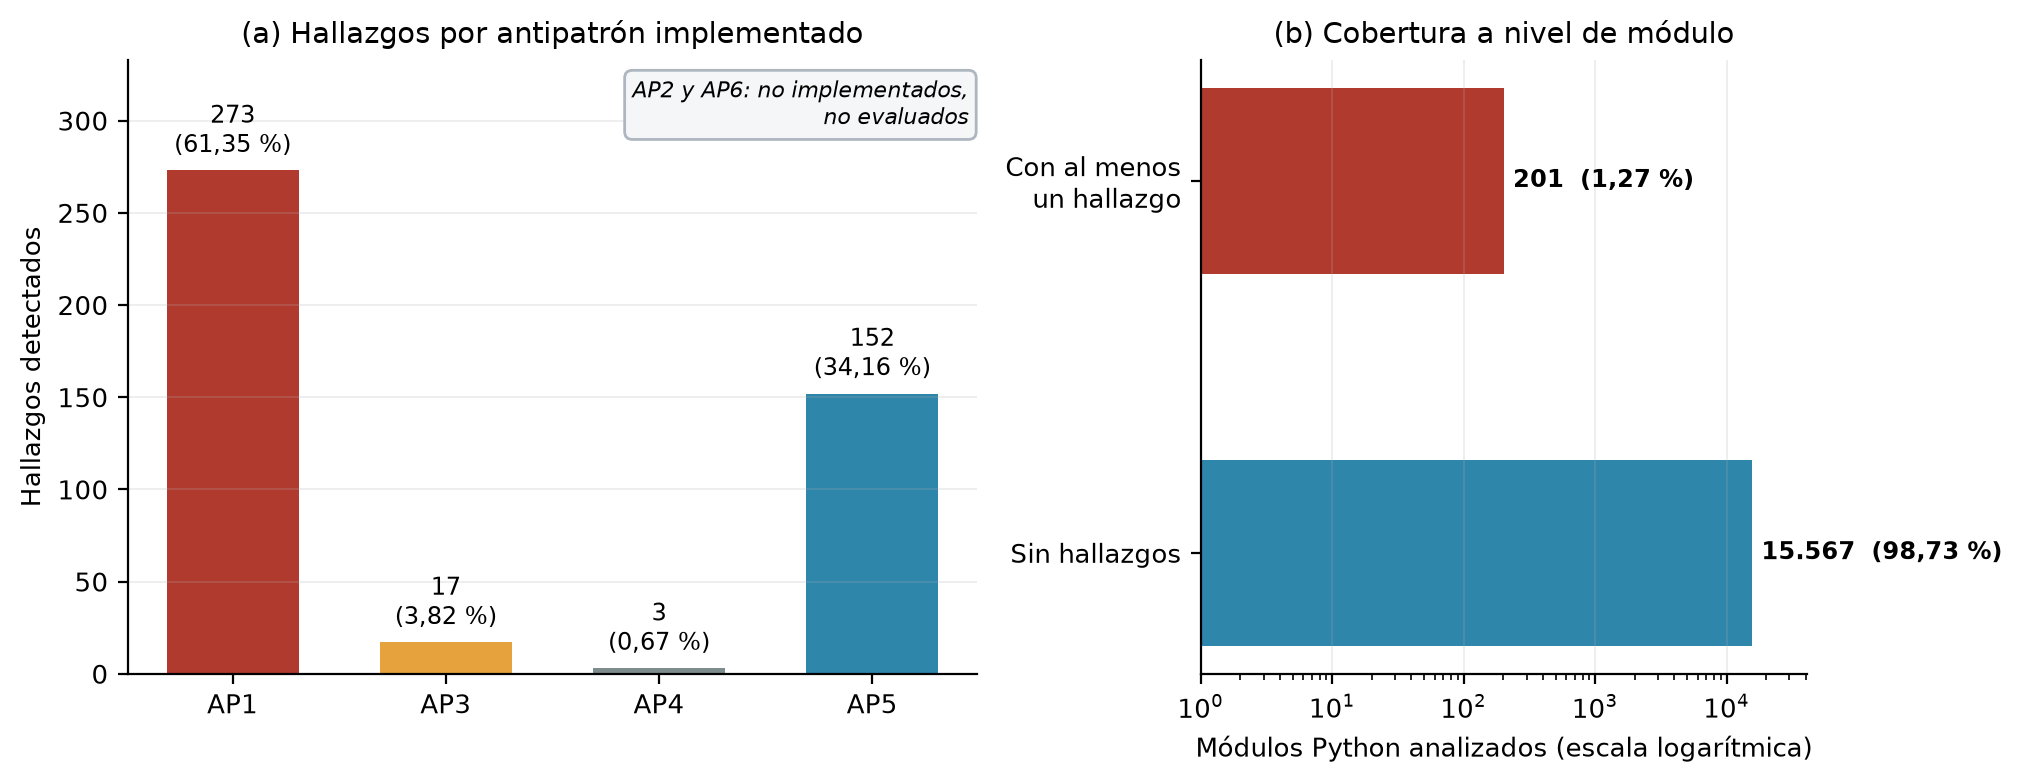
\includegraphics[width=0.92\textwidth]{figuras/fig03_distribucion_hallazgos.png}
\caption{Distribución de los hallazgos. (a) Hallazgos por antipatrón implementado; AP2 y AP6 no fueron implementados y no se evaluaron. (b) Módulos con y sin al menos un hallazgo, en escala logarítmica.}
\label{fig:distribucion}
\end{figure*}

\subsection{Organización y tabulación}

La información se organizó en archivos con granularidad explícita. El nivel de repositorio se conserva en \texttt{repos\_seleccionados.csv} y en \texttt{resumen\_repositorio.csv}; el nivel de módulo, en \texttt{metricas.csv}; el nivel de hallazgo, en \texttt{findings.csv}; y el nivel de análisis, en \texttt{estadisticas.csv}, \texttt{spearman.csv}, \texttt{resumen\_descriptivo.csv} y \texttt{decisiones\_hipotesis.csv}. La clave de unión entre hallazgos y métricas es la pareja \texttt{(repo, file)}, con rutas relativas a la raíz del repositorio. La matriz repositorio por antipatrón se conserva en \texttt{tabla\_repo\_ap.csv}, y la revisión asistida por IA en \texttt{validacion\_investigador.csv}.

La tabulación siguió tres reglas. Primero, no se agregaron filas ni se imputaron valores: los conteos de hallazgos, módulos y repositorios se derivan directamente de los archivos. Segundo, las métricas se calcularon una sola vez por módulo y se reutilizaron en todos los análisis. Tercero, las decisiones estadísticas se registraron en un archivo separado con sus criterios, entradas, resultado y limitaciones, de modo que la conclusión no dependiera de una interpretación posterior. La auditoría de consistencia verificó que no hay hallazgos sin métricas, que no hay claves duplicadas y que no hay valores faltantes en las métricas primarias.

\subsection{Presentación de los resultados}

El orden de presentación sigue la lógica del análisis. Primero se describe el volumen y la composición de la muestra. Luego se presenta la distribución de los antipatrones y su concentración por repositorio. A continuación se reportan los descriptivos de las métricas y el contraste primario entre grupos. Después se presentan las correlaciones, el análisis por terciles de tamaño y la sensibilidad por repositorio. Finalmente se reporta la revisión asistida por IA con su alcance limitado. Esta secuencia permite que el lector reconstruya el razonamiento antes de llegar a la discusión y a las conclusiones, y evita que los resultados se presenten como una colección de valores sin relación con las preguntas de investigación.